\chapter{Interacțiunea cu mediul extern}

\section{Interfața serială}

\label{sec:InterfataSeriala}

Este foarte probabil ca mulți dintre voi să fi depanat până acum un program software doar prin folosirea metodei clasice și probabil cea mai simplă și intuitivă - folosirea \textit{printf-urilor} (limbajul C) sau a \textit{cout-urilor} dacă sunteți familarizați cu C++. Dacă în cadrul unei aplicații software clasice, ieșirea programului este redată pe un monitor, în cadrul unei aplicații embedded nu avem un astfel de dispozitiv. Cel mult vom avea un LCD. În acest caz, ne propunem să trimitem aceste date către un calculator personal prin care le-am putea accesa cu ușurință. Soluția este folosirea unei interfețe seriale. Configurația oferită de către proiectul inițial (folosind \textit{Processor Expert}) are deja inițializată interfața serială de pe microcontroller.

Aceasta poate fi folosita din programul dezvoltat pe microcontroller prin apelul următoarelor funcții:

\begin{description}
    \item[void Term1\_SendChar(char\_t Val)] Realizează transmiterea unui singur caracter.
    \item[void Term1\_SendStr(void *str)] Util pentru transmiterea unui șir de caractere (a unui string).
    \item[void Term1\_SendNum(int32\_t number)] Util pentru transmiterea unui număr întreg (reprezentat pe 32 de biți).
\end{description}

\begin{figure}[h!]
  \vspace{-10pt}
  \center{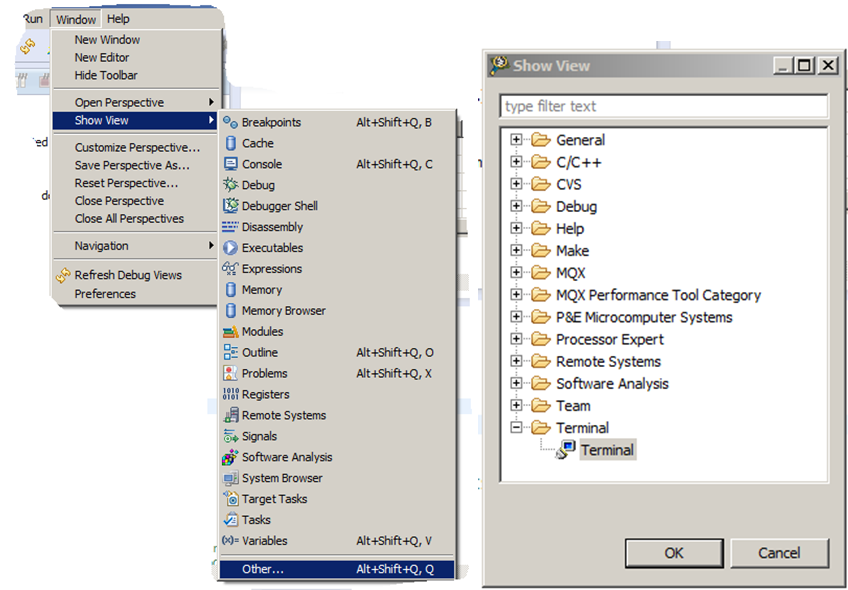
\includegraphics[width=0.8 \textwidth]{images/EclipseTerminal.png}}
  \vspace{-5pt}
  \caption{\label{fig:CodeWarrior-EclipseTerminal} Accesarea terminalului pus la dispoziție de Eclipse}
  \vspace{-10pt}
\end{figure}

În mediul de dezvoltare (Eclipse) se poate folosi un terminal pentru a recepționa datele transmise de către microcontroller prin interfața serială. Acest terminal va trebui accesat ca în figura \ref{fig:CodeWarrior-EclipseTerminal}.

Terminalul va apărea în partea de jos a ecranului în taburile de console. Pentru o comunicare corectă (pentru ca terminalul să înțeleagă corect datele trimise), terminalul trebuie configurat după cum urmează:

Portul selectat trebuie să fie portul pe care s-a atașat \textit{OpenSDA} (în Windows, poate fi verificat în \textit{"Device Manager"}, mai exact în \textit{"Ports (COM \& LPT)"}). După configurare, terminalul va trebui conectat la portul cu care comunică. Aceasta se face prin simpla apăsare a butonului de conectare (primul din lista de butoane de tip iconițe ale ferestrei "Terminal" ce apare în partea de jos a Eclipse-ului).

\section{Senzori cu infraroșu}

Pentru a putea detecta diferența dintre linia neagră și fundalul alb al traseului, robotul \textit{Zumo} folosește o matrice de senzori cu infraroșu. Acești senzori pot măsura cantitatea de lumina reflectată de diferite suprafațe, în funcție de proprietățile acesteia. Cum funcționează? Foarte simplu. O diodă emite radiații în spectrul infraroșu spre suprafața din dreptul senzorului și o parte mai mică sau mai mare din această lumina va fi absorbită de suprafață. Ce ne interesează pe noi este cantitea de lumina reflectată ce va fi masurată cu ajutorul unui fototranzistor și al unui condensator.

\begin{wrapfigure}{l}{0.5\textwidth}
    \vspace{-20pt}
    \center{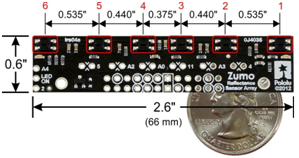
\includegraphics[width=0.5 \textwidth]{images/InfraredSensors.png}}
    \vspace{-15pt}
    \caption{\label{fig:CodeWarrior-InfraredSensors} Bareta de senzori}
    \vspace{-20pt}
\end{wrapfigure}

După cum îi spune și numele, matricea de senzori este alcătuită din mai multe elemente. Acest lucru este necesar deoarece fiecare senzor poate măsura doar cantitatea de lumina care este reflectată din jurul său (pe o arie redusă ca și suprafață). Bareta care este pusă la dispoziție pentru robotul Zumo are 6 astfel de elemente pentru detecția liniei negre. Aceasta este amplasată sub lama robotului, asigurându-se o protecție atât mecanică cât și o reducere a cantității de lumina ambientală care poate duce la perturbarea măsurătorilor.

Ieșirea senzorilor este dată de durata ($T$) a unui impuls electric. Cu cât impulsul este mai de durată, cu atât cantitatea de lumina reflectată este mai mică.

Următoarele componente \textit{Processor Expert} vor fi folosite în interfațarea cu acești senzori:

\begin{itemize}
    \item intrările / ieșirile digitale (componente de tip \textit{BitIO}): A1, A3, D11, A0, A2, D5, IR\_LED;
    \item un timer (componentă de tip \textit{TimerUnit\_LDD}) CountTimer;
    \item componentă necesară adăugării unui întârzieri - \textit{WAIT1};
\end{itemize}

Pașii necesari pentru obținerea unei iterații de date despre mediu, de la senzori, ar fi următorii:

\begin{enumerate}
    \item Activăm diodele infraroșii - IR\_LED.
    \item Configurăm pinii digitali (A1, A3, D11, A0, A2, D5) ca ieșiri și le setăm pe valoarea 1.
    \item Așteptăm o perioadă de timp astfel încât condensatorul să se încarce - 50 µs este suficient.
    \item Configurăm pinii de la pasul 2 ca intrări digitale (adică pini de input), de această dată.
    \item Resetăm timer-ul \textit{CountTimer}. După inițializare acesta va funcționa în mod continuu și va număra la infinit, motiv pentru care avem nevoie de o resetare a acestuia la intervale periodice de timp. Resetarea va asigura faptul că numărătoarea începe de la 0. Timer-ul măsoară perioade de timp în multipli de 6.10 µs (163.84kHz).
    \item Măsurăm timpul necesar ca tensiunea de pe condensator să comute intrările în valoarea 0. După o perioadă de câteva µs, senzorii pot fi considerați ca au toți valoarea 0. Acest mecanism ne permite să reducem perioada de așteptare între citiri, după un anumit prag (perioadă) nu se mai obțin informatii utile de la senzori.
    \item Dezactivăm diodele infraroșii.
\end{enumerate}

Toate modulele prezentate pe scurt în cadrul acestui capitol, se pot interconecta folosind schema din Figura 1 de la secțiunea \textit{~\nameref{sec:AnexaInterconectare}}, anexată la acest document.